
\usepackage[round,authoryear]{natbib}
\usepackage{paralist}
\usepackage{pgfpages}
\usepackage{mathtools}
\usepackage{amsmath}
\usepackage{amssymb}
\usepackage{xspace}        
\usepackage{graphicx}

\bibliographystyle{jss}

\usefonttheme[onlymath]{serif}
% use article-like math letters, from http://tex.stackexchange.com/questions/34265/how-to-get-beamer-math-to-look-like-article-math

\newcommand\prob[1]{\mathbb{P}\left[{#1}\right]}
\newcommand\expect[1]{\mathbb{E}\left[{#1}\right]}
\newcommand\var[1]{\mathrm{Var}\left[{#1}\right]}
\newcommand\dist[2]{\mathrm{#1}\left(#2\right)}
\newcommand\dlta[1]{{\Delta}{#1}}
\newcommand\lik{\mathcal{L}}
\newcommand\loglik{\ell}
\newcommand\R{\mathbb{R}}
\newcommand\Rzero{\mathfrak{R}_0}
\newcommand\argmax{\mathop{\mathrm{argmax}}}
\newcommand\argmin{\mathop{\mathrm{argmin}}}

\newcommand\code[1]{\texttt{#1}}
\newcommand\package[1]{\textbf{#1}}

\newcommand\link[2]{\href{#1}{#2}}
\newcommand{\doi}[1]{\link{https://doi.org/#1}{\texttt{doi:~{#1}}}}

\newcommand{\scinot}[2]{#1{\times}10^{#2}}
\newcommand{\dd}[1]{\mathrm{d}{#1}}
\newcommand{\pd}[3][]{%
  \def\ord{#1} \ifx\ord\empty%
  \frac{\partial{#2}}{\partial{#3}}%
  \else \frac{\partial^{#1}{#2}}{\partial{#3}^{#1}}%
  \fi
}
\newcommand{\deriv}[3][]{%
  \def\ord{#1} \ifx\ord\empty%
  \frac{\dd{#2}}{\dd{#3}}%
  \else \frac{\dd^{#1}{#2}}{\dd{#3}^{#1}}%
  \fi
}

\newcommand\Rlanguage{\textsf{R}\xspace}

\newcommand\question{{\bf Question}}
\newcommand\mysolution{{\bf Solution}}
\newcounter{Qcounter}
\newcommand\myquestion{{\stepcounter{Qcounter} Question \CHAPTER.\theQcounter}}
\newcounter{Ecounter}
\newcommand\myexercise{{\stepcounter{Ecounter} Exercise \CHAPTER.\theEcounter}}

\newcommand\myexample{{\bf Example}}
\newcommand\mydot{{\,\cdot\,}}
\newcommand\myref[1]{\m{#1}}

\newcommand\Rspace{\mathcal{R}}

\renewcommand\vec[1]{\boldsymbol{\mathrm{#1}}}
\newcommand\vect[1]{\vec{#1}}
\newcommand\mat[1]{\mathbb{#1}}
\newcommand\pr{\mathbb{P}}
\newcommand\E{\mathbb{E}}

\newcommand\profileloglik[1]{\ell^\mathrm{profile}_#1}
\newcommand\Real{\mathbb{R}}

\newcommand\bi{\begin{itemize}}
\newcommand\ei{\end{itemize}}

\newcommand\normal{\mathrm{normal}}

\newcommand\iid{\mathrm{iid}}
\newcommand\MVN{\mathrm{MVN}}
\newcommand\SE{\mathrm{SE}}

\newcommand\pval{\mathrm{pval}}
% \newcommand\var{\mathrm{Var}}
\newcommand\sd{\mathrm{SD}}
\newcommand\sdSample{\mathrm{sd}}
\newcommand\varSample{\mathrm{var}}
\newcommand\cov{\mathrm{Cov}}
\newcommand\covSample{\mathrm{cov}}
\newcommand\corSample{\mathrm{cor}}
\newcommand\cor{\mathrm{Cor}}
\newcommand\given{{\, | \,}}
\newcommand\param{\,;}
\newcommand\params{\param}
\newcommand\equals{{ \, = \, }}
\newcommand\transpose{{\raisebox{0.5mm}{\mbox{\scriptsize \textsc{t}}}}}
%\newcommand\transpose{\scriptsize{T}}
\newcommand\mycolon{{\hspace{0.5mm}:\hspace{0.5mm}}}
%\newcommand\mycolon{\,{:}\,}
\newcommand\myemph[1]{{\textbf{#1}}}
\newcommand\mymathenv[1]{\textcolor{blue}{#1}}


%% following a style where all math is in blue
%% not currently used by SISMID slides
\newcommand\mymath[1]{\begin{math}\textcolor{blue}{#1}\end{math}}
\newcommand\m[1]{\mymath{#1}}
\newcommand\mydisplaymath[1]{\begin{displaymath}\textcolor{blue}{#1}\end{displaymath}}
\newcommand\myeqnarray[1]{\textcolor{blue}{\begin{eqnarray*}#1 \end{eqnarray*}}}
\newcommand\myspace{\quad}
\newcommand\altdisplaymath[1]{\vspace{1mm}\textcolor{blue}{\begin{math}\displaystyle #1 \end{math}}\vspace{1mm}}


%% not currently used in SISMID slides.
%% a plain and space-efficient list useful for dense slides
%% the compactenum and compactitem environments from paralist are probably prefer%% able
%% \newcommand\enumerateSpace{\hspace{2mm}}
%% \newenvironment {myitemize} {
%%                  \begin{list}{\textcolor{black}{$\bullet$} \hfill}
%%                  {\setlength{\labelwidth}{0.3 cm}
%%                   \setlength{\leftmargin}{0.15cm}
%%                   \setlength{\itemindent}{0.15cm}
%%                   \setlength{\labelsep}{0cm}
%%                   \setlength{\parsep}{0.2 ex}
%%                   \setlength{\itemsep}{1 mm}
%%       \setlength{\topsep}{0.0cm}}} %space between title and 1st item
%%    {\end{list}}

\setlength{\parskip}{0mm}
\setlength{\parindent}{0mm}

\newcommand\negBeforeCode{}
\newcommand\negAfterCode{}

\mode<beamer>{\usetheme{AnnArbor}}
\mode<beamer>{\setbeamertemplate{footline}}
\mode<beamer>{\setbeamertemplate{footline}[frame number]}
\mode<beamer>{\setbeamertemplate{frametitle continuation}[from second][\insertcontinuationcountroman]}
\mode<beamer>{\setbeamertemplate{navigation symbols}{}}

\mode<handout>{\pgfpagesuselayout{2 on 1}[letterpaper,border shrink=5mm]}



\mode<beamer>{\usetheme{AnnArbor}}
\mode<beamer>{\setbeamertemplate{footline}}
\mode<beamer>{\setbeamertemplate{footline}[frame number]}
\mode<beamer>{\setbeamertemplate{frametitle continuation}[from second][\insertcontinuationcountroman]}
\mode<beamer>{\setbeamertemplate{navigation symbols}{}}

\mode<handout>{\pgfpagesuselayout{2 on 1}[letterpaper,border shrink=5mm]}

\title{Lesson 6:\\Case study: Polio}
\author{Aaron A. King, Edward L. Ionides and Kidus Asfaw}


\newcommand\CHAPTER{6}

% \setbeamertemplate{footline}[frame number]

\newcommand\eqspace{\quad\quad\quad}
\newcommand\eqskip{\vspace{2.5mm}}

\newcommand\dist[2]{\mathrm{#1}\left(#2\right)}
\newcommand\dlta{\Delta}

\newcommand\myeq{\hspace{10mm}}

% \newcommand\answer[2]{\textcolor{blue}{#2}} % to show answers
% \newcommand\answer[2]{{\color{blue}{#2}}} % to show answers
\newcommand\answer[2]{#1} % to show blank space



\usepackage{bbm} % for blackboard bold 1

\begin{document}

% knitr set up









\begin{frame}
  \titlepage
\end{frame}

\begin{frame}{Outline}
  \tableofcontents
\end{frame}


\begin{frame}{Objectives}
%\frametitle{Chapter \CHAPTER. Case study: Polio}

%\hspace{3cm} {\large \bf Objectives}

%\vspace{3mm}

\begin{enumerate}

\item Demonstrate the use of covariates in \package{pomp} to add demographic data (birth rates and total population) and  seasonality to an epidemiological model.

\item Show how partially observed Markov process (POMP) models and methods can be used to understand transmission dynamics of polio.

\item Practice maximizing the likelihood for such models. How to set up a global search for a maximum likelihood estimate. How to assess whether a search has been successful.

\item Provide a workflow that can be adapted to related data analysis tasks.

\end{enumerate}

\end{frame}

\section{Covariates}

\begin{frame}{Reviewing covariates in time series analysis}

\bi

\item Suppose our time series of primary interest is $y_{1:N}$.

\item A \myemph{covariate} time series is an additional time series ${z_{1:N}}$ which is used to help explain $y_{1:N}$.

\item When we talk about covariates, it is often implicit that we think of ${z_{1:N}}$ as a measure of an \myemph{external forcing} to the system producing $y_{1:N}$. This means that the process generating the data ${z_{1:N}}$ affects the process generating $y_{1:N}$, but not vice versa. 

 \item For example, the weather might affect human health, but human health has negligible effect on weather: weather is an external forcing to human health processes.

\item When the process leading to  ${z_{1:N}}$ is not external to the system generating it, we must be alert to the possibility of \myemph{reverse causation} and \myemph{confounding variables}.

\ei

\end{frame}

\begin{frame}[fragile]

\frametitle{Including covariates in the general POMP framework}

\bi
\item The general POMP modeling framework allows essentially arbitrary modeling of covariates.

\item Recall that a POMP model is specified by defining, for $n=1:N$,
$$\begin{array}{l}
f_{X_{0}}(x_0\params\theta),
\\
f_{X_{n}|X_{n-1}}(x_{n}\given x_{n-1}\params\theta),
\\
f_{Y_{n}|X_n}(y_{n}\given x_n\params\theta).
\end{array}$$

\item The possibility of a general dependence on $n$ includes the possibility that there is some covariate time series $z_{0:N}$ such that
$$\begin{array}{lcl}
f_{X_{0}}(x_0\params\theta)&=& f_{X_{0}}(x_0\params\theta,z_0)
\\
f_{X_{n}|X_{n-1}}(x_{n}\given x_{n-1}\params\theta) &=& f_{X_{n}|X_{n-1}}(x_{n}\given x_{n-1}\params\theta,z_n),
\\
f_{Y_{n}|X_n}(y_{n}\given x_n\params\theta) &=& f_{Y_{n}|X_n}(y_{n}\given x_n\params\theta,z_n).
\end{array}$$

\ei

\end{frame}

\begin{frame}[fragile]

\frametitle{Seasonality in a POMP model}

\bi

\item One specific choice of covariates is to construct $z_{0:N}$ so that it fluctuates periodically, once per year. This allows \myemph{seasonality} enter the POMP model in whatever way is appropriate for the system under investigation.

\item All that remains is to hypothesize what is a reasonable way to include covariates for your system, and to fit the resulting model.

\item Now we can evaluate and maximize the log likelihood, we can construct AIC or likelihood ratio tests to see if the covariate helps describe the data.

\item This also lets us compare alternative ways the covariates might enter the process model and/or the measurement model.

\ei

\end{frame}

\begin{frame}[fragile]


\frametitle{Covariates in the \package{pomp} package}

\bi

\item \package{pomp} provides facilities for including covariates in a pomp object.

\item Named covariate time series entered via the \code{covar} argument to \code{pomp} are automatically defined within Csnippets used for the \code{rprocess}, \code{dprocess}, \code{rmeasure}, \code{dmeasure} and \code{rinit} arguments.

\item We see this in practice in the following epidemiological model, which has  population census, birth data and seasonality as covariates.

\ei

\end{frame}

\section{A POMP model for polio}

\begin{frame}[fragile]

\frametitle{Polio in Wisconsin}

\bi

\item The massive global polio eradication initiative (GPEI) has brought polio from a major global disease to the brink of extinction. 

\item Finishing this task is proving hard, and improved understanding polio ecology might assist.  

\item \citet{Martinez-Bakker2015} investigated this using extensive state level pre-vaccination era data in USA. 

\item We will follow the approach of \citet{Martinez-Bakker2015} for one state (Wisconsin). In the context of their model, we can quantify seasonality of transmission, the role of the birth rate in explaining the transmission dynamics, and the persistence mechanism of polio. 


\ei

\end{frame}

\begin{frame}[fragile]

\bi
\item \citet{Martinez-Bakker2015} carried out this analysis for all 48 contigous states and District of Columbia, and their data and code are publicly available. The data we study, in \code{polio_wisconsin.csv}, consist of \code{cases}, the monthly reported polio cases; \code{births}, the  monthly recorded births; \code{pop}, the annual census; \code{time}, date in years.
\ei

\begin{knitrout}\small
\definecolor{shadecolor}{rgb}{0.969, 0.969, 0.969}\color{fgcolor}\begin{kframe}
\begin{alltt}
\hlstd{polio_data} \hlkwb{<-} \hlkwd{read.csv}\hlstd{(}\hlstr{"polio_wisconsin.csv"}\hlstd{,}\hlkwc{comment}\hlstd{=}\hlstr{"#"}\hlstd{)}
\hlkwd{head}\hlstd{(polio_data,}\hlnum{5}\hlstd{)}
\end{alltt}
\begin{verbatim}
##       time cases births     pop
## 1 1931.083     7   4698 2990000
## 2 1931.167     0   4354 2990000
## 3 1931.250     7   4836 2990000
## 4 1931.333     3   4468 2990000
## 5 1931.417     4   4712 2990000
\end{verbatim}
\end{kframe}
\end{knitrout}

\end{frame}

\begin{frame}[fragile]

\begin{knitrout}\small
\definecolor{shadecolor}{rgb}{0.969, 0.969, 0.969}\color{fgcolor}

{\centering \includegraphics[width=12cm]{tmp/figuredata_plot-1} 

}



\end{knitrout}


\end{frame}

\begin{frame}[fragile]

\bi

\item We use the compartment model of \citet{Martinez-Bakker2015}.

\item Compartments representing susceptible babies in each of six one-month birth cohorts ($S^B_1$,...,$S^B_6$), susceptible older individuals ($S^O$), infected babies ($I^B$), infected older individuals ($I^O$), and recovered with lifelong immunity ($R$). 

\item The state vector of the disease transmission model consists of numbers of individuals in each compartment at each time, 
$$X(t)=\big(S^B_1(t),...,S^B_6(t), I^B(t),I^O(t),R(t) \big).$$

\item Babies under six months are modeled as fully protected from symptomatic poliomyelitis.

\item Older infections lead to reported cases (usually paralysis) at a rate $\rho$. 

\item The flows through the compartments are graphically represented on the following slide (Figure 1A of \citet{Martinez-Bakker2015}):

\ei

\end{frame}

\begin{frame}[fragile]

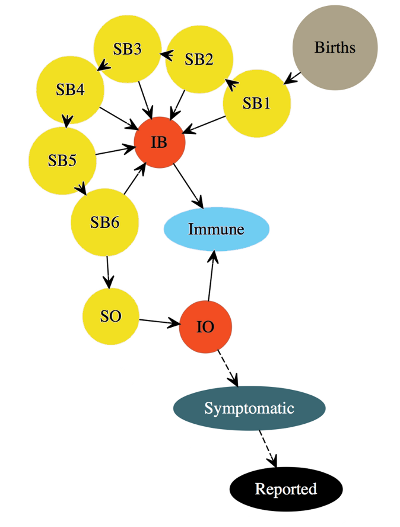
\includegraphics[width=6cm]{polio_fig1A.png} \hspace{-5mm}\parbox[b]{5.5cm}{
SBk, suscepbible babies $k$ months\\
IB, infected babies\\
SO, susceptible older people\\
IO, infected older people

\vspace{3cm}

}

\end{frame}

\begin{frame}[fragile]

\frametitle{Setting up the model}

\bi

\item Duration of infection is comparable to the one-month reporting aggregation, so a discrete time model may be appropriate.

\item \citet{Martinez-Bakker2015} fitted monthly reported cases, May 1932 through January 1953, so we set $t_n=1932+ (4+n)/12$ and
$$X_n=X(t_n)=\big(S^B_{1,n},...,S^B_{6,n}, I^B_n,I^O_n,R_n \big).$$

\item The mean force of infection, in units of $\mathrm{yr}^{-1}$, is modeled as
$$\bar\lambda_n=\left( \beta_n \frac{I^O_n+I^B_n}{P_n} + \psi \right)$$
where $P_n$ is census population interpolated to time $t_n$ and seasonality of transmission is modeled as
$$\beta_n=\exp\left\{ \sum_{k=1}^K b_k\xi_k(t_n) \right\},$$
with $\{\xi_k(t),k=1,\dots,K\}$ a periodic B-spline basis with $K=6$.

\item $P_n$ and $\xi_k(t_n)$ are \myemph{covariate time series}.

\ei

\end{frame}

\begin{frame}[fragile]

\bi
\item The force of infection has a stochastic perturbation,
$$\lambda_n = \bar\lambda_n \epsilon_n,$$
where $\epsilon_n$ is a Gamma random variable with mean 1 and variance $\sigma^2_{\mathrm{env}} + \sigma^2_{\mathrm{dem}}\big/\bar\lambda_n$. These two terms capture variation on the environmental and demographic scales, respectively. All compartments suffer a mortality rate, set at $\delta=1/60\mathrm{yr}^{-1}$. 

\item Within each month, all susceptible individuals are modeled as having exposure to constant competing hazards of mortality and polio infection.  The chance of remaining in the susceptible population when exposed to these hazards for one month is therefore
$$p_n = \exp\big\{ -(\delta+\lambda_n)/12\big\},$$
with the chance of polio infection being 
$$q_n = (1-p_n)\lambda_n\big/(\lambda_n+\delta).$$

\ei

\end{frame}

\begin{frame}

\bi
\item We employ a continuous population model, with no demographic stochasticity. Writing $B_n$ for births in month $n$, we obtain the dynamic model of \citet{Martinez-Bakker2015}:
$$\begin{array}{rcl}
S^B_{1,n+1}&=&B_{n+1}\\
S^B_{k,n+1}&=&p_nS^B_{k-1,n} \quad\mbox{for $k=2,\dots,6$}\\
S^O_{n+1}&=& p_n(S^O_n+S^B_{6,n})\\
I^B_{n+1}&=& q_n \sum_{k=1}^6 S^B_{k,n}\\
I^O_{n+1}&=& q_n S^O_n
\end{array}$$
\ei

\end{frame}

\begin{frame}[fragile]
\frametitle{The measurement model}

\bi
\item 
The model for the reported observations, conditional on the state, is a discretized normal distribution truncated at zero, with both environmental and Poisson-scale contributions to the variance:
$$Y_n= \max\{\mathrm{round}(Z_n),0\}, \quad Z_n\sim\mathrm{normal}\left(\rho I^O_n, \big(\tau  I^O_n\big)^2 + \rho I^O_n\right).$$
\ei

\end{frame}

\begin{frame}[fragile]

\frametitle{Initial conditions}

\bi
\item 
Additional parameters are used to specify initial state values at time $t_0=1932+ 4/12$.
\item 
We will suppose there are parameters $\big(\tilde S^B_{1,0},...,\tilde S^B_{6,0}, \tilde I^B_0,\tilde I^O_0,\tilde S^O_0\big)$ that specify the population in each compartment at time $t_0$ via
$$ S^B_{1,0}= {\tilde S}^B_{1,0} ,...,S^B_{6,0}= \tilde S^B_{6,0}, \quad I^B_{0}= P_0 \tilde I^B_{0},\quad S^O_{0}= P_0 \tilde S^O_{0}, \quad I^O_{0}= P_0 \tilde I^O_{0}.$$
\item
Following \citet{Martinez-Bakker2015}, we make an approximation for the initial conditions of ignoring infant infections at time $t_0$. 
Thus, we set $\tilde I^B_{0}=0$ and use monthly births in the preceding months (ignoring infant mortality) to fix $\tilde S^B_{k,0}=B_{1-k}$ for $k=1,\dots,6$. The estimated initial conditions are then defined by the two parameters $\tilde I^O_{0}$ and $\tilde S^O_{0}$, since the initial recovered population, $R_0$, is specified by subtraction of all the other compartments from the total initial population, $P_0$.
\item 
It is convenient to parameterize the estimated initial states as fractions of the population, whereas the initial states fixed at births are parameterized directly as a count.

\ei

\end{frame}

\section{A \texttt{pomp} representation of the POMP model}

\begin{frame}[fragile]

\frametitle{Building a \code{pomp} object for the polio model}

\bi
\item
We code the state and observation variables, and the choice of $t_0$, as
\ei

\begin{knitrout}\small
\definecolor{shadecolor}{rgb}{0.969, 0.969, 0.969}\color{fgcolor}\begin{kframe}
\begin{alltt}
\hlstd{polio_statenames} \hlkwb{<-} \hlkwd{c}\hlstd{(}\hlstr{"SB1"}\hlstd{,}\hlstr{"SB2"}\hlstd{,}\hlstr{"SB3"}\hlstd{,}\hlstr{"SB4"}\hlstd{,}\hlstr{"SB5"}\hlstd{,}\hlstr{"SB6"}\hlstd{,}
  \hlstr{"IB"}\hlstd{,}\hlstr{"SO"}\hlstd{,}\hlstr{"IO"}\hlstd{)}
\hlstd{polio_obsnames} \hlkwb{<-} \hlstr{"cases"}
\hlstd{polio_t0} \hlkwb{<-} \hlnum{1932}\hlopt{+}\hlnum{4}\hlopt{/}\hlnum{12}
\end{alltt}
\end{kframe}
\end{knitrout}
\bi
\item 
We do not explictly code $R$, since it is defined implicitly as the total population minus the sum of the other compartments. Due to lifelong immunity, individuals in $R$ play no role in the dynamics. Even occasional negative values of $R$ (due to a discrepancy between the census and the mortality model) would not be a fatal flaw.
\ei
\end{frame}

\begin{frame}[fragile]

\frametitle{Setting up the covariate table}
\bi
\item
\code{time} gives the time at which the covariates are defined.
\item
\code{P} is a smoothed interpolation of the annual census.
\item
\code{B} is monthly births.
\item \code{xi1,...,xi6}  is a periodic B-spline basis
\ei

\begin{knitrout}\small
\definecolor{shadecolor}{rgb}{0.969, 0.969, 0.969}\color{fgcolor}\begin{kframe}
\begin{alltt}
\hlstd{polio_K} \hlkwb{<-} \hlnum{6}
\hlstd{polio_covar} \hlkwb{<-} \hlkwd{covariate_table}\hlstd{(}
  \hlkwc{t}\hlstd{=polio_data}\hlopt{$}\hlstd{time,}
  \hlkwc{B}\hlstd{=polio_data}\hlopt{$}\hlstd{births,}
  \hlkwc{P}\hlstd{=}\hlkwd{predict}\hlstd{(}\hlkwd{smooth.spline}\hlstd{(}\hlkwc{x}\hlstd{=}\hlnum{1931}\hlopt{:}\hlnum{1954}\hlstd{,}
    \hlkwc{y}\hlstd{=polio_data}\hlopt{$}\hlstd{pop[}\hlkwd{seq}\hlstd{(}\hlnum{12}\hlstd{,}\hlnum{24}\hlopt{*}\hlnum{12}\hlstd{,}\hlkwc{by}\hlstd{=}\hlnum{12}\hlstd{)]))}\hlopt{$}\hlstd{y,}
  \hlkwd{periodic.bspline.basis}\hlstd{(t,}\hlkwc{nbasis}\hlstd{=polio_K,}
    \hlkwc{degree}\hlstd{=}\hlnum{3}\hlstd{,}\hlkwc{period}\hlstd{=}\hlnum{1}\hlstd{,}\hlkwc{names}\hlstd{=}\hlstr{"xi%d"}\hlstd{),}
  \hlkwc{times}\hlstd{=}\hlstr{"t"}
\hlstd{)}
\end{alltt}
\end{kframe}
\end{knitrout}

\end{frame}

\begin{frame}[fragile]
\frametitle{Regular parameters and initial value parameters}

\bi
\item
The parameters $b_1,\dots,b_\mathrm{K},\psi,\rho,\tau,\sigma_\mathrm{dem}, \sigma_\mathrm{env}$  in the model above are {regular parameters} (RPs), coded as
\ei
\begin{knitrout}\small
\definecolor{shadecolor}{rgb}{0.969, 0.969, 0.969}\color{fgcolor}\begin{kframe}
\begin{alltt}
\hlstd{polio_rp_names} \hlkwb{<-} \hlkwd{c}\hlstd{(}\hlstr{"b1"}\hlstd{,}\hlstr{"b2"}\hlstd{,}\hlstr{"b3"}\hlstd{,}\hlstr{"b4"}\hlstd{,}\hlstr{"b5"}\hlstd{,}\hlstr{"b6"}\hlstd{,}
  \hlstr{"psi"}\hlstd{,}\hlstr{"rho"}\hlstd{,}\hlstr{"tau"}\hlstd{,}\hlstr{"sigma_dem"}\hlstd{,}\hlstr{"sigma_env"}\hlstd{)}
\end{alltt}
\end{kframe}
\end{knitrout}

\bi
\item
The {initial value parameters} (IVPs), $\tilde I^O_{0}$ and  $\tilde S^O_{0}$, are coded for each state named by adding \code{_0} to the state name:
\ei
\begin{knitrout}\small
\definecolor{shadecolor}{rgb}{0.969, 0.969, 0.969}\color{fgcolor}\begin{kframe}
\begin{alltt}
\hlstd{polio_ivp_names} \hlkwb{<-} \hlkwd{c}\hlstd{(}\hlstr{"SO_0"}\hlstd{,}\hlstr{"IO_0"}\hlstd{)}
\hlstd{polio_paramnames} \hlkwb{<-} \hlkwd{c}\hlstd{(polio_rp_names,polio_ivp_names)}
\end{alltt}
\end{kframe}
\end{knitrout}

\end{frame}

\begin{frame}[fragile]

\frametitle{Fixed parameters (FPs)}
\bi
\item 
Two quantities in the dynamic model specification, $\delta=1/60 \mathrm{yr}^{-1}$ and $\mathrm{K}=6$, are not estimated.
\item Six other initial value quantities, $\{\tilde S^B_{1,0},\dots,\tilde S^B_{6,0}\}$, are treated as fixed.

\item Fixed quantities could be coded as constants using the \code{globals} argument of \code{pomp}, but here we pass them as fixed parameters (FPs).
\ei

\begin{knitrout}\small
\definecolor{shadecolor}{rgb}{0.969, 0.969, 0.969}\color{fgcolor}\begin{kframe}
\begin{alltt}
\hlstd{polio_fp_names} \hlkwb{<-} \hlkwd{c}\hlstd{(}\hlstr{"delta"}\hlstd{,}\hlstr{"K"}\hlstd{,}
  \hlstr{"SB1_0"}\hlstd{,}\hlstr{"SB2_0"}\hlstd{,}\hlstr{"SB3_0"}\hlstd{,}\hlstr{"SB4_0"}\hlstd{,}\hlstr{"SB5_0"}\hlstd{,}\hlstr{"SB6_0"}\hlstd{)}
\hlstd{polio_paramnames} \hlkwb{<-} \hlkwd{c}\hlstd{(polio_rp_names,}
  \hlstd{polio_ivp_names,polio_fp_names)}
\hlstd{covar_index_t0} \hlkwb{<-} \hlkwd{which}\hlstd{(}\hlkwd{abs}\hlstd{(polio_covar}\hlopt{@}\hlkwc{times}\hlopt{-}\hlstd{polio_t0)}\hlopt{<}\hlnum{0.01}\hlstd{)}
\hlstd{polio_initial_births} \hlkwb{<-} \hlstd{polio_covar}\hlopt{@}\hlkwc{table}\hlstd{[}\hlstr{"B"}\hlstd{,covar_index_t0}\hlopt{-}\hlnum{0}\hlopt{:}\hlnum{5}\hlstd{]}
\hlkwd{names}\hlstd{(polio_initial_births)} \hlkwb{<-} \hlkwd{c}\hlstd{(}\hlstr{"SB1_0"}\hlstd{,}\hlstr{"SB2_0"}\hlstd{,}
  \hlstr{"SB3_0"}\hlstd{,}\hlstr{"SB4_0"}\hlstd{,}\hlstr{"SB5_0"}\hlstd{,}\hlstr{"SB6_0"}\hlstd{)}
\hlstd{polio_fixed_params} \hlkwb{<-} \hlkwd{c}\hlstd{(}\hlkwc{delta}\hlstd{=}\hlnum{1}\hlopt{/}\hlnum{60}\hlstd{,}\hlkwc{K}\hlstd{=polio_K,}
  \hlstd{polio_initial_births)}
\end{alltt}
\end{kframe}
\end{knitrout}

\end{frame}

\begin{frame}[fragile]

\frametitle{A starting value for the parameters}

\bi
\item We have to start somewhere for our search in parameter space.
\item The following parameter vector is based on informal model exploration and prior research:
\ei

\begin{knitrout}\small
\definecolor{shadecolor}{rgb}{0.969, 0.969, 0.969}\color{fgcolor}\begin{kframe}
\begin{alltt}
\hlstd{polio_params_guess} \hlkwb{<-} \hlkwd{c}\hlstd{(}\hlkwc{b1}\hlstd{=}\hlnum{3}\hlstd{,}\hlkwc{b2}\hlstd{=}\hlnum{0}\hlstd{,}\hlkwc{b3}\hlstd{=}\hlnum{1.5}\hlstd{,}\hlkwc{b4}\hlstd{=}\hlnum{6}\hlstd{,}\hlkwc{b5}\hlstd{=}\hlnum{5}\hlstd{,}\hlkwc{b6}\hlstd{=}\hlnum{3}\hlstd{,}
  \hlkwc{psi}\hlstd{=}\hlnum{0.002}\hlstd{,}\hlkwc{rho}\hlstd{=}\hlnum{0.01}\hlstd{,}\hlkwc{tau}\hlstd{=}\hlnum{0.001}\hlstd{,}\hlkwc{sigma_dem}\hlstd{=}\hlnum{0.04}\hlstd{,}\hlkwc{sigma_env}\hlstd{=}\hlnum{0.5}\hlstd{,}
  \hlkwc{SO_0}\hlstd{=}\hlnum{0.12}\hlstd{,}\hlkwc{IO_0}\hlstd{=}\hlnum{0.001}\hlstd{,polio_fixed_params)}
\end{alltt}
\end{kframe}
\end{knitrout}

\end{frame}

\begin{frame}[fragile]

\begin{knitrout}\small
\definecolor{shadecolor}{rgb}{0.969, 0.969, 0.969}\color{fgcolor}\begin{kframe}
\begin{alltt}
\hlstd{polio_rprocess} \hlkwb{<-} \hlkwd{Csnippet}\hlstd{(}\hlstr{"
  double beta = exp(dot_product( (int) K, &xi1, &b1));
  double lambda = (beta * (IO+IB) / P + psi);
  double var_epsilon = pow(sigma_dem,2)/ lambda +  
    pow(sigma_env,2);
  lambda *= (var_epsilon < 1.0e-6) ? 1 : 
    rgamma(1/var_epsilon,var_epsilon);
  double p = exp(- (delta+lambda)/12);
  double q = (1-p)*lambda/(delta+lambda);
  SB1 = B;
  SB2= SB1*p;
  SB3=SB2*p;
  SB4=SB3*p;
  SB5=SB4*p;
  SB6=SB5*p;
  SO= (SB6+SO)*p;
  IB=(SB1+SB2+SB3+SB4+SB5+SB6)*q;
  IO=SO*q;
"}\hlstd{)}
\end{alltt}
\end{kframe}
\end{knitrout}

\end{frame}

\begin{frame}[fragile]

\begin{knitrout}\small
\definecolor{shadecolor}{rgb}{0.969, 0.969, 0.969}\color{fgcolor}\begin{kframe}
\begin{alltt}
\hlstd{polio_dmeasure} \hlkwb{<-} \hlkwd{Csnippet}\hlstd{(}\hlstr{"
  double tol = 1.0e-25;
  double mean_cases = rho*IO;
  double sd_cases = sqrt(pow(tau*IO,2) + mean_cases);
  if(cases > 0.0)\{
    lik = pnorm(cases+0.5,mean_cases,sd_cases,1,0)
      - pnorm(cases-0.5,mean_cases,sd_cases,1,0) + tol; 
  \} else\{
    lik = pnorm(cases+0.5,mean_cases,sd_cases,1,0) + tol;
  \}
  if (give_log) lik = log(lik);
"}\hlstd{)}

\hlstd{polio_rmeasure} \hlkwb{<-} \hlkwd{Csnippet}\hlstd{(}\hlstr{"
  cases = rnorm(rho*IO, sqrt( pow(tau*IO,2) + rho*IO ) );
  if (cases > 0.0) \{
    cases = nearbyint(cases);
  \} else \{
    cases = 0.0;
  \}
"}\hlstd{)}
\end{alltt}
\end{kframe}
\end{knitrout}

\end{frame}

\begin{frame}[fragile]

The map from the initial value parameters to the initial value of the states at time $t_0$ is coded by the \code{rinit} function:

\begin{knitrout}\small
\definecolor{shadecolor}{rgb}{0.969, 0.969, 0.969}\color{fgcolor}\begin{kframe}
\begin{alltt}
\hlstd{polio_rinit} \hlkwb{<-} \hlkwd{Csnippet}\hlstd{(}\hlstr{"
  SB1 = SB1_0;
  SB2 = SB2_0;
  SB3 = SB3_0;
  SB4 = SB4_0;
  SB5 = SB5_0;
  SB6 = SB6_0;
  IB = 0;
  IO = IO_0 * P;
  SO = SO_0 * P;
"}\hlstd{)}
\end{alltt}
\end{kframe}
\end{knitrout}

\end{frame}

\begin{frame}[fragile]

\frametitle{Parameter transformations}
\bi
\item For parameter estimation, it is helpful to have transformations that map each parameter into the whole real line and which put uncertainty close to a unit scale
\ei
\begin{knitrout}\small
\definecolor{shadecolor}{rgb}{0.969, 0.969, 0.969}\color{fgcolor}\begin{kframe}
\begin{alltt}
\hlstd{polio_partrans} \hlkwb{<-} \hlkwd{parameter_trans}\hlstd{(}
  \hlkwc{log}\hlstd{=}\hlkwd{c}\hlstd{(}\hlstr{"psi"}\hlstd{,}\hlstr{"rho"}\hlstd{,}\hlstr{"tau"}\hlstd{,}\hlstr{"sigma_dem"}\hlstd{,}\hlstr{"sigma_env"}\hlstd{),}
  \hlkwc{logit}\hlstd{=}\hlkwd{c}\hlstd{(}\hlstr{"SO_0"}\hlstd{,}\hlstr{"IO_0"}\hlstd{)}
\hlstd{)}
\end{alltt}
\end{kframe}
\end{knitrout}
\bi
\item Since the seasonal splines are exponentiated, the \code{beta} parameters are already defined on the real line with unit scale uncertainty.
\ei

\end{frame}

\begin{frame}[fragile]

We now put these pieces together into a pomp object. 
\begin{knitrout}\small
\definecolor{shadecolor}{rgb}{0.969, 0.969, 0.969}\color{fgcolor}\begin{kframe}
\begin{alltt}
\hlstd{polio} \hlkwb{<-} \hlkwd{pomp}\hlstd{(}
  \hlkwc{data}\hlstd{=}\hlkwd{subset}\hlstd{(polio_data,}
    \hlstd{(time} \hlopt{>} \hlstd{polio_t0} \hlopt{+} \hlnum{0.01}\hlstd{)} \hlopt{&} \hlstd{(time} \hlopt{<} \hlnum{1953}\hlopt{+}\hlnum{1}\hlopt{/}\hlnum{12}\hlopt{+}\hlnum{0.01}\hlstd{),}
    \hlkwc{select}\hlstd{=}\hlkwd{c}\hlstd{(}\hlstr{"cases"}\hlstd{,}\hlstr{"time"}\hlstd{)),}
  \hlkwc{times}\hlstd{=}\hlstr{"time"}\hlstd{,}
  \hlkwc{t0}\hlstd{=polio_t0,}
  \hlkwc{params}\hlstd{=polio_params_guess,}
  \hlkwc{rprocess} \hlstd{=} \hlkwd{euler}\hlstd{(}\hlkwc{step.fun} \hlstd{= polio_rprocess,} \hlkwc{delta.t}\hlstd{=}\hlnum{1}\hlopt{/}\hlnum{12}\hlstd{),}
  \hlkwc{rmeasure}\hlstd{= polio_rmeasure,}
  \hlkwc{dmeasure} \hlstd{= polio_dmeasure,}
  \hlkwc{covar}\hlstd{=polio_covar,}
  \hlkwc{obsnames} \hlstd{= polio_obsnames,}
  \hlkwc{statenames} \hlstd{= polio_statenames,}
  \hlkwc{paramnames} \hlstd{= polio_paramnames,}
  \hlkwc{rinit}\hlstd{=polio_rinit,}
  \hlkwc{partrans}\hlstd{=polio_partrans}
\hlstd{)}
\end{alltt}
\end{kframe}
\end{knitrout}

\end{frame}

\section{Logistics for the computations}

\subsection*{Controlling run time}

\begin{frame}[fragile]

\frametitle{Setting run levels to control computation time}

\bi

\item \code{run_level=1} will set all the algorithmic parameters to the first column of values in the following code, for debugging.

\item Here, \code{Np} is the number of particles, \code{Nmif} is the number of iterations of the optimization procedure carried, other variables are defined for use later.

\item \code{run_level=2} uses enough effort to gives reasonably stable results at a moderate computational time.

\item Larger values give more refined computations, implemented here by \code{run_level=3} which was run on a computing node.

\ei

\begin{knitrout}\small
\definecolor{shadecolor}{rgb}{0.969, 0.969, 0.969}\color{fgcolor}\begin{kframe}
\begin{alltt}
\hlstd{run_level} \hlkwb{<-} \hlnum{1}
\hlstd{polio_Np} \hlkwb{<-}          \hlkwd{switch}\hlstd{(run_level,}\hlnum{100}\hlstd{,} \hlnum{1e3}\hlstd{,} \hlnum{5e3}\hlstd{)}
\hlstd{polio_Nmif} \hlkwb{<-}        \hlkwd{switch}\hlstd{(run_level,} \hlnum{10}\hlstd{,} \hlnum{100}\hlstd{,} \hlnum{200}\hlstd{)}
\hlstd{polio_Nreps_eval} \hlkwb{<-}  \hlkwd{switch}\hlstd{(run_level,}  \hlnum{2}\hlstd{,}  \hlnum{10}\hlstd{,}  \hlnum{20}\hlstd{)}
\hlstd{polio_Nreps_local} \hlkwb{<-} \hlkwd{switch}\hlstd{(run_level,} \hlnum{10}\hlstd{,}  \hlnum{20}\hlstd{,}  \hlnum{40}\hlstd{)}
\hlstd{polio_Nreps_global} \hlkwb{<-}\hlkwd{switch}\hlstd{(run_level,} \hlnum{10}\hlstd{,}  \hlnum{20}\hlstd{,} \hlnum{100}\hlstd{)}
\hlstd{polio_Nsim} \hlkwb{<-}        \hlkwd{switch}\hlstd{(run_level,} \hlnum{50}\hlstd{,} \hlnum{100}\hlstd{,} \hlnum{500}\hlstd{)}
\end{alltt}
\end{kframe}
\end{knitrout}

\end{frame}

\begin{frame}[fragile]

\frametitle{Comments on setting algorithmic parameters}

\bi

\item Using \code{run_level} settings is convenient for editing source code. It plays no fundamental role in the final results. If you are not editing the source code, or using the code as a template for developing your own analysis, it has no function.

\item When you edit a document with different \code{run_level} options, you can debug your code by editing \code{run_level=1}. Then, you can get preliminary assessment of whether your results are sensible with \code{run_level=2} and get finalized results, with reduced Monte Carlo error, by editing \code{run_level=3}.

\item We intend \code{run_level=1} to run in minutes, \code{run_level=2} to run in tens of minutes, and \code{run_level=3} to run in hours.

\item You can increase or decrease the numbers of particles, or the number of mif2 iterations, or the number of global searches carried out, to make sure this procedure is practical on your machine.
 
\item Appropriate values of the algorithmic parameters for each run-level are context dependent.

\ei

\end{frame}

\begin{frame}[fragile]

\myexercise. \myemph{Choosing algorithmic parameters}.\\
Suppose you have selected a number of particles, \code{Np}, and number of iterated filtering iterations, \code{Nmif}, and number of Monte Carlo replications, \code{Reps}, that give a 10 minute maximization search using \code{mif2()}. Propose how you would adjust these to plan a more intensive search lasting about 2 hours.

\answer{\vspace{40mm}}{todo}

\end{frame}

\subsection*{Parallel computation of the likelihood}

\begin{frame}[fragile]

\frametitle{Parallel set-up}

\bi
\item
As discussed in earlier lessons, we ask {\Rlanguage} to access multiple processors and we set up a parallel random number generator.
\ei

\begin{knitrout}\small
\definecolor{shadecolor}{rgb}{0.969, 0.969, 0.969}\color{fgcolor}\begin{kframe}
\begin{alltt}
\hlkwd{library}\hlstd{(doParallel)}
\hlkwd{registerDoParallel}\hlstd{(}\hlkwd{detectCores}\hlstd{())}
\hlkwd{library}\hlstd{(doRNG)}
\hlkwd{registerDoRNG}\hlstd{(}\hlnum{3899882}\hlstd{)}
\end{alltt}
\end{kframe}
\end{knitrout}

\bi
\item Our task, like most statistical computing, is \myemph{embarrassingly parallel}.
\item Therefore, we can use a simple parallel for loop via \code{foreach()}
\ei
\end{frame}


\begin{frame}[fragile]

\frametitle{Likelihood evaluation at the starting parameter estimate}


\begin{knitrout}\small
\definecolor{shadecolor}{rgb}{0.969, 0.969, 0.969}\color{fgcolor}\begin{kframe}
\begin{alltt}
\hlkwd{stew}\hlstd{(}\hlkwc{file}\hlstd{=}\hlkwd{sprintf}\hlstd{(}\hlstr{"results/pf1-%d.rda"}\hlstd{,run_level),\{}
  \hlstd{t1} \hlkwb{<-} \hlkwd{system.time}\hlstd{(}
    \hlstd{pf1} \hlkwb{<-} \hlkwd{foreach}\hlstd{(}\hlkwc{i}\hlstd{=}\hlnum{1}\hlopt{:}\hlnum{20}\hlstd{,}\hlkwc{.packages}\hlstd{=}\hlstr{'pomp'}\hlstd{)} \hlopt \hlkwd{pfilter}\hlstd{(}
      \hlstd{polio,}\hlkwc{Np}\hlstd{=polio_Np)}
  \hlstd{)}
\hlstd{\})}
\hlstd{L1} \hlkwb{<-} \hlkwd{logmeanexp}\hlstd{(}\hlkwd{sapply}\hlstd{(pf1,logLik),}\hlkwc{se}\hlstd{=}\hlnum{TRUE}\hlstd{)}
\end{alltt}
\end{kframe}
\end{knitrout}

\bi

\item In  2.7 seconds, we obtain a log likelihood estimate of -826.33 with a Monte standard error of 0.92.

\item Here, we use \code{stew()} to \myemph{cache} the results of the computation.
\ei

\end{frame}

\subsection*{Caching results}

\begin{frame}[fragile]
\frametitle{Caching computations in Rmarkdown}

\bi

\item  It is not unusual for computations in a POMP analysis to take hours to run on many cores.

\item  The computations for a final version of a manuscript may take days.

\item  Usually, we use some mechanism like the different values of \code{run_level} so that preliminary versions of the manuscript take less time to run.

\item  However, when editing the text or working on a different part of the manuscript, we don't want to re-run long pieces of code.

\item  Saving results so that the code is only re-run when necessary is called \myemph{caching}.

\ei

\end{frame}

\begin{frame}[fragile]
\bi
\item  You may already be familiar the versions of caching provided in {.Rmd} and {.Rnw} files. The argument \code{cache=TRUE} can be set individually for each chunk or as a global option.

\item  When \code{cache=TRUE}, Rmarkdown/knitr caches the results of the chunk, meaning that a chunk will only be re-run if code in that chunk is edited.

\item  You can force Rmarkdown/knitr to recompute all the chunks by deleting the \code{cache} subdirectory.
\ei
\end{frame}


\begin{frame}[fragile]
\frametitle{Practical advice for caching}
\bi
\item  What if changes elsewhere in the document affect the proper evaluation of your chunk, but you didn't edit any of the code in the chunk itself?
Rmarkdown/knitr will get this wrong. \myemph{It will not recompute the chunk}.

\item  A perfect caching system doesn't exist. \myemph{Always delete the entire cache and rebuild a fresh cache before finishing a manuscript.}

\item  Rmarkdown/knitr caching is good for relatively small computations, such as producing figures or things that may take a minute or two and are annoying if you have to recompute them every time you make any edits to the text.

\item  For longer computations, it is good to have full manual control. In \package{pomp}, this is provided by two related functions, \code{stew} and \code{bake}.

\ei

\end{frame}

\begin{frame}[fragile]

\frametitle{\code{stew} and \code{bake}}
\bi
\item  Notice the function \code{stew} in the replicated particle filter code above.

\item  Here, \code{stew} looks for a file called \code{pf-[run_level].rda}. 

\item  If it finds this file, it simply loads the contents of this file.

\item  If the file doesn't exist, it carries out the specified computation and saves it in a file of this name.

\item  \code{bake} is similar to \code{stew}. The difference is that \code{bake} uses \code{readRDS} and \code{saveRDS}, whereas \code{stew} uses \code{load} and \code{save}. 

\item  either way, the computation will not be re-run unless you manually delete \code{pf-[run_level].rda}.

\item  \code{stew} and \code{bake} reset the seed appropriately whether or not the computation is recomputed. Othewise, caching risks adverse consequences for reproducibility.

\ei

\end{frame}   

\section{Persistence of polio}

\begin{frame}[fragile]

\frametitle{Simulation to investigate local persistence}

\bi
\item 
The scientific purpose of fitting a model typically involves analyzing properties of the fitted model, often investigated using simulation.
\item Following \citet{Martinez-Bakker2015}, we are interested in how often months with no reported cases ($Y_n=0$) correspond to months without any local asymptomatic cases, defined for our continuous state model as $I^B_n+I^O_n<1/2$.
\item For Wisconsin, using our model at the estimated MLE, we simulate in parallel as follows:
\ei
\begin{knitrout}\small
\definecolor{shadecolor}{rgb}{0.969, 0.969, 0.969}\color{fgcolor}\begin{kframe}
\begin{alltt}
\hlkwd{stew}\hlstd{(}\hlkwd{sprintf}\hlstd{(}\hlstr{"results/persistence-%d.rda"}\hlstd{,run_level),\{}
  \hlstd{t_sim} \hlkwb{<-} \hlkwd{system.time}\hlstd{(}
    \hlstd{sim} \hlkwb{<-} \hlkwd{foreach}\hlstd{(}\hlkwc{i}\hlstd{=}\hlnum{1}\hlopt{:}\hlstd{polio_Nsim,}
      \hlkwc{.packages}\hlstd{=}\hlstr{'pomp'}\hlstd{)} \hlopt \hlkwd{simulate}\hlstd{(polio)}
  \hlstd{)}
\hlstd{\})}
\end{alltt}
\end{kframe}
\end{knitrout}

\end{frame}
\begin{frame}[fragile]

\begin{knitrout}\small
\definecolor{shadecolor}{rgb}{0.969, 0.969, 0.969}\color{fgcolor}\begin{kframe}
\begin{alltt}
\hlstd{no_cases_data} \hlkwb{<-} \hlkwd{sum}\hlstd{(}\hlkwd{obs}\hlstd{(polio)}\hlopt{==}\hlnum{0}\hlstd{)}
\hlstd{no_cases_sim} \hlkwb{<-} \hlkwd{sum}\hlstd{(}\hlkwd{sapply}\hlstd{(sim,obs)}\hlopt{==}\hlnum{0}\hlstd{)}\hlopt{/}\hlkwd{length}\hlstd{(sim)}
\hlstd{fadeout1_sim} \hlkwb{<-} \hlkwd{sum}\hlstd{(}\hlkwd{sapply}\hlstd{(sim,}\hlkwa{function}\hlstd{(}\hlkwc{po}\hlstd{)}\hlkwd{states}\hlstd{(po)[}\hlstr{"IB"}\hlstd{,]}
  \hlopt{+}\hlkwd{states}\hlstd{(po)[}\hlstr{"IO"}\hlstd{,]}\hlopt{<}\hlnum{1}\hlstd{))}\hlopt{/}\hlkwd{length}\hlstd{(sim)}
\hlstd{fadeout100_sim} \hlkwb{<-} \hlkwd{sum}\hlstd{(}\hlkwd{sapply}\hlstd{(sim,}\hlkwa{function}\hlstd{(}\hlkwc{po}\hlstd{)}\hlkwd{states}\hlstd{(po)[}\hlstr{"IB"}\hlstd{,]}
  \hlopt{+}\hlkwd{states}\hlstd{(po)[}\hlstr{"IO"}\hlstd{,]}\hlopt{<}\hlnum{100}\hlstd{))}\hlopt{/}\hlkwd{length}\hlstd{(sim)}
\hlstd{imports_sim} \hlkwb{<-} \hlkwd{coef}\hlstd{(polio)[}\hlstr{"psi"}\hlstd{]}\hlopt{*}\hlkwd{mean}\hlstd{(}\hlkwd{sapply}\hlstd{(sim,}
  \hlkwa{function}\hlstd{(}\hlkwc{po}\hlstd{)} \hlkwd{mean}\hlstd{(}\hlkwd{states}\hlstd{(po)[}\hlstr{"SO"}\hlstd{,]}\hlopt{+}\hlkwd{states}\hlstd{(po)[}\hlstr{"SB1"}\hlstd{,]}
    \hlopt{+}\hlkwd{states}\hlstd{(po)[}\hlstr{"SB2"}\hlstd{,]}\hlopt{+}\hlkwd{states}\hlstd{(po)[}\hlstr{"SB3"}\hlstd{,]}\hlopt{+}\hlkwd{states}\hlstd{(po)[}\hlstr{"SB4"}\hlstd{,]}
    \hlopt{+}\hlkwd{states}\hlstd{(po)[}\hlstr{"SB5"}\hlstd{,]}\hlopt{+}\hlkwd{states}\hlstd{(po)[}\hlstr{"SB6"}\hlstd{,])))}\hlopt{/}\hlnum{12}
\end{alltt}
\end{kframe}
\end{knitrout}

\vspace{-1mm}

 For the data, there were 26 months with no reported cases, similar to the mean of 50.4 for simulations from the fitted model. Months with no asyptomatic infections for the simulations were rare, on average 0.7 months per simulation. Months with fewer than 100 infections averaged 64.4 per simulation, which in the context of a reporting rate of 0.01 can explain the absences of case reports. The mean monthly infections due to importations, modeled by $\psi$, is 117.1. This does not give much opportunity for local elimination of poliovirus.
 
\end{frame}
\begin{frame}[fragile]

\bi
\item It is also good practice to look at simulations from the fitted model:

\ei

\begin{knitrout}\small
\definecolor{shadecolor}{rgb}{0.969, 0.969, 0.969}\color{fgcolor}\begin{kframe}
\begin{alltt}
\hlstd{mle_simulation} \hlkwb{<-} \hlkwd{simulate}\hlstd{(polio,}\hlkwc{seed}\hlstd{=}\hlnum{127}\hlstd{)}
\hlkwd{plot}\hlstd{(mle_simulation)}
\end{alltt}
\end{kframe}

{\centering \includegraphics[width=\maxwidth]{tmp/figureplot_simulated-1} 

}



\end{knitrout}

\end{frame}

\begin{frame}[fragile]

\bi

\item We see from this simulation that the fitted model can generate report histories that look qualitatively similar to the data. However, there are things to notice in the reconstructed latent states. Specifically, the pool of older susceptibles, $S^O(t)$, is mostly increasing. The reduced case burden in the data in the time interval 1932--1945 is explained by a large initial recovered ($R$) population, which implies much higher levels of polio before 1932. There were large epidemics of polio in the USA early in the 20th century, so this is not implausible.

\item A liklihood profile over the parameter $\tilde S^O_0$ could help to clarify to what extent this is a critical feature of how the model explains the data.

\ei

\end{frame}

\section{Likelihood maximization}

\begin{frame}[fragile]

\frametitle{Local likelihood maximization}

\bi

\item Let's see if we can improve on the previous MLE. We use the IF2 algorithm. We set a constant random walk standard deviation for each of the regular parameters and a larger constant for each of the initial value parameters:

\ei
\begin{knitrout}\small
\definecolor{shadecolor}{rgb}{0.969, 0.969, 0.969}\color{fgcolor}\begin{kframe}
\begin{alltt}
\hlstd{polio_rw.sd_rp} \hlkwb{<-} \hlnum{0.02}
\hlstd{polio_rw.sd_ivp} \hlkwb{<-} \hlnum{0.2}
\hlstd{polio_cooling.fraction.50} \hlkwb{<-} \hlnum{0.5}
\hlstd{polio_rw.sd} \hlkwb{<-} \hlkwd{rw.sd}\hlstd{(}
  \hlkwc{b1}\hlstd{=polio_rw.sd_rp,}\hlkwc{b2}\hlstd{=polio_rw.sd_rp,}\hlkwc{b3}\hlstd{=polio_rw.sd_rp,}
  \hlkwc{b4}\hlstd{=polio_rw.sd_rp,}\hlkwc{b5}\hlstd{=polio_rw.sd_rp,}\hlkwc{b6}\hlstd{=polio_rw.sd_rp,}
  \hlkwc{psi}\hlstd{=polio_rw.sd_rp,} \hlkwc{rho}\hlstd{=polio_rw.sd_rp,}
  \hlkwc{tau}\hlstd{=polio_rw.sd_rp,} \hlkwc{sigma_dem}\hlstd{=polio_rw.sd_rp,}
  \hlkwc{sigma_env}\hlstd{=polio_rw.sd_rp,}
  \hlkwc{IO_0}\hlstd{=}\hlkwd{ivp}\hlstd{(polio_rw.sd_ivp),} \hlkwc{SO_0}\hlstd{=}\hlkwd{ivp}\hlstd{(polio_rw.sd_ivp)}
\hlstd{)}
\end{alltt}
\end{kframe}
\end{knitrout}

\end{frame}

\begin{frame}[fragile]

\begin{knitrout}\small
\definecolor{shadecolor}{rgb}{0.969, 0.969, 0.969}\color{fgcolor}\begin{kframe}
\begin{alltt}
\hlkwd{stew}\hlstd{(}\hlkwd{sprintf}\hlstd{(}\hlstr{"results/mif-%d.rda"}\hlstd{,run_level),\{}
  \hlstd{t2} \hlkwb{<-} \hlkwd{system.time}\hlstd{(\{}
    \hlstd{m2} \hlkwb{<-} \hlkwd{foreach}\hlstd{(}\hlkwc{i}\hlstd{=}\hlnum{1}\hlopt{:}\hlstd{polio_Nreps_local,}
      \hlkwc{.packages}\hlstd{=}\hlstr{'pomp'}\hlstd{,} \hlkwc{.combine}\hlstd{=c)} \hlopt \hlkwd{mif2}\hlstd{(polio,}
           \hlkwc{Np}\hlstd{=polio_Np,}
           \hlkwc{Nmif}\hlstd{=polio_Nmif,}
           \hlkwc{cooling.fraction.50}\hlstd{=polio_cooling.fraction.50,}
           \hlkwc{rw.sd}\hlstd{=polio_rw.sd)}
    \hlstd{lik_m2} \hlkwb{<-} \hlkwd{foreach}\hlstd{(}\hlkwc{i}\hlstd{=}\hlnum{1}\hlopt{:}\hlstd{polio_Nreps_local,}
      \hlkwc{.packages}\hlstd{=}\hlstr{'pomp'}\hlstd{,} \hlkwc{.combine}\hlstd{=rbind)} \hlopt \hlkwd{logmeanexp}\hlstd{(}
        \hlkwd{replicate}\hlstd{(polio_Nreps_eval,}\hlkwd{logLik}\hlstd{(}
          \hlkwd{pfilter}\hlstd{(polio,}\hlkwc{params}\hlstd{=}\hlkwd{coef}\hlstd{(m2[[i]]),}\hlkwc{Np}\hlstd{=polio_Np))),}
        \hlkwc{se}\hlstd{=}\hlnum{TRUE}\hlstd{)}
  \hlstd{\})}
\hlstd{\})}
\end{alltt}
\end{kframe}
\end{knitrout}

\end{frame}

\begin{frame}[fragile]

\begin{knitrout}\small
\definecolor{shadecolor}{rgb}{0.969, 0.969, 0.969}\color{fgcolor}\begin{kframe}
\begin{alltt}
\hlstd{r2} \hlkwb{<-} \hlkwd{data.frame}\hlstd{(}\hlkwc{logLik}\hlstd{=lik_m2[,}\hlnum{1}\hlstd{],}\hlkwc{logLik_se}\hlstd{=lik_m2[,}\hlnum{2}\hlstd{],}
  \hlkwd{t}\hlstd{(}\hlkwd{sapply}\hlstd{(m2,coef)))}
\hlstd{polio_results} \hlkwb{<-} \hlkwd{read.table}\hlstd{(}\hlstr{"polio_params_in.csv"}\hlstd{,}
  \hlkwc{row.names}\hlstd{=}\hlkwa{NULL}\hlstd{,}\hlkwc{header}\hlstd{=T)}
\hlkwd{write.table}\hlstd{(}\hlkwd{rbind}\hlstd{(polio_results,r2),}
  \hlkwc{file}\hlstd{=}\hlstr{"polio_params_out.csv"}\hlstd{,}\hlkwc{row.names}\hlstd{=}\hlnum{FALSE}\hlstd{)}
\hlkwd{summary}\hlstd{(r2}\hlopt{$}\hlstd{logLik,}\hlkwc{digits}\hlstd{=}\hlnum{5}\hlstd{)}
\end{alltt}
\begin{verbatim}
##    Min. 1st Qu.  Median    Mean 3rd Qu.    Max. 
## -2015.3 -1061.2  -859.8 -1044.9  -820.1  -813.4
\end{verbatim}
\end{kframe}
\end{knitrout}

\bi

\item This investigation took  0.2 minutes.
\item
These repeated stochastic maximizations can also show us the geometry of the likelihood surface in a neighborhood of this point estimate:

\ei

\end{frame}

\begin{frame}[fragile]
\begin{knitrout}\small
\definecolor{shadecolor}{rgb}{0.969, 0.969, 0.969}\color{fgcolor}\begin{kframe}
\begin{alltt}
\hlkwd{pairs}\hlstd{(}\hlopt{~}\hlstd{logLik}\hlopt{+}\hlstd{psi}\hlopt{+}\hlstd{rho}\hlopt{+}\hlstd{tau}\hlopt{+}\hlstd{sigma_dem}\hlopt{+}\hlstd{sigma_env,}
  \hlkwc{data}\hlstd{=}\hlkwd{subset}\hlstd{(r2,logLik}\hlopt{>}\hlkwd{max}\hlstd{(logLik)}\hlopt{-}\hlnum{20}\hlstd{))}
\end{alltt}
\end{kframe}

{\centering \includegraphics[width=\maxwidth]{tmp/figurepairs-1} 

}



\end{knitrout}

\end{frame}

\begin{frame}[fragile]

\bi

\item We see strong tradeoffs between $\psi$, $\rho$ and $\sigma_\mathrm{dem}$. By itself, in the absence of other assumptions, the pathogen immigration rate $\psi$ is fairly weakly identified. However, the reporting rate $\rho$ is essentially the fraction of poliovirus infections leading to acute flaccid paralysis, which is known to be around 1\%. This plot suggests that fixing an assumed value of $\rho$ might lead to much more precise inference on $\psi$; the rate of pathogen immigration presumably being important for understanding disease persistence. These hypotheses could be investigated more formally by construction of profile likelihood plots and likelihood ratio tests.

\ei

\end{frame}

\begin{frame}[fragile]

\frametitle{Global likelihood maximization}

\bi
\item 
Practical parameter estimation involves trying many starting values for the parameters. One can specify a large box in parameter space that contains all sensible parameter vectors.

\item If the estimation gives stable conclusions with starting values drawn randomly from this box, we have some confidence that our global search is reliable.

\item For our polio model, a reasonable box might be:
\ei

\begin{knitrout}\small
\definecolor{shadecolor}{rgb}{0.969, 0.969, 0.969}\color{fgcolor}\begin{kframe}
\begin{alltt}
\hlstd{polio_box} \hlkwb{<-} \hlkwd{rbind}\hlstd{(}
  \hlkwc{b1}\hlstd{=}\hlkwd{c}\hlstd{(}\hlopt{-}\hlnum{2}\hlstd{,}\hlnum{8}\hlstd{),} \hlkwc{b2}\hlstd{=}\hlkwd{c}\hlstd{(}\hlopt{-}\hlnum{2}\hlstd{,}\hlnum{8}\hlstd{),}
  \hlkwc{b3}\hlstd{=}\hlkwd{c}\hlstd{(}\hlopt{-}\hlnum{2}\hlstd{,}\hlnum{8}\hlstd{),} \hlkwc{b4}\hlstd{=}\hlkwd{c}\hlstd{(}\hlopt{-}\hlnum{2}\hlstd{,}\hlnum{8}\hlstd{),}
  \hlkwc{b5}\hlstd{=}\hlkwd{c}\hlstd{(}\hlopt{-}\hlnum{2}\hlstd{,}\hlnum{8}\hlstd{),} \hlkwc{b6}\hlstd{=}\hlkwd{c}\hlstd{(}\hlopt{-}\hlnum{2}\hlstd{,}\hlnum{8}\hlstd{),}
  \hlkwc{psi}\hlstd{=}\hlkwd{c}\hlstd{(}\hlnum{0}\hlstd{,}\hlnum{0.1}\hlstd{),} \hlkwc{rho}\hlstd{=}\hlkwd{c}\hlstd{(}\hlnum{0}\hlstd{,}\hlnum{0.1}\hlstd{),} \hlkwc{tau}\hlstd{=}\hlkwd{c}\hlstd{(}\hlnum{0}\hlstd{,}\hlnum{0.1}\hlstd{),}
  \hlkwc{sigma_dem}\hlstd{=}\hlkwd{c}\hlstd{(}\hlnum{0}\hlstd{,}\hlnum{0.5}\hlstd{),} \hlkwc{sigma_env}\hlstd{=}\hlkwd{c}\hlstd{(}\hlnum{0}\hlstd{,}\hlnum{1}\hlstd{),}
  \hlkwc{SO_0}\hlstd{=}\hlkwd{c}\hlstd{(}\hlnum{0}\hlstd{,}\hlnum{1}\hlstd{),} \hlkwc{IO_0}\hlstd{=}\hlkwd{c}\hlstd{(}\hlnum{0}\hlstd{,}\hlnum{0.01}\hlstd{)}
\hlstd{)}
\end{alltt}
\end{kframe}
\end{knitrout}


\end{frame}


\begin{frame}[fragile]

We then carry out a search identical to the local one except for the starting parameter values. This can be succinctly coded by calling \code{mif2} on the previously constructed object, \code{m2[[1]]}, with a reset starting value:

\begin{knitrout}\small
\definecolor{shadecolor}{rgb}{0.969, 0.969, 0.969}\color{fgcolor}\begin{kframe}
\begin{alltt}
\hlkwd{stew}\hlstd{(}\hlkwc{file}\hlstd{=}\hlkwd{sprintf}\hlstd{(}\hlstr{"results/box_eval-%d.rda"}\hlstd{,run_level),\{}
  \hlstd{t3} \hlkwb{<-} \hlkwd{system.time}\hlstd{(\{}
    \hlstd{m3} \hlkwb{<-} \hlkwd{foreach}\hlstd{(}\hlkwc{i}\hlstd{=}\hlnum{1}\hlopt{:}\hlstd{polio_Nreps_global,}\hlkwc{.packages}\hlstd{=}\hlstr{'pomp'}\hlstd{,}
      \hlkwc{.combine}\hlstd{=c)} \hlopt \hlkwd{mif2}\hlstd{(}
        \hlstd{m2[[}\hlnum{1}\hlstd{]],}
        \hlkwc{params}\hlstd{=}\hlkwd{c}\hlstd{(}\hlkwd{apply}\hlstd{(polio_box,}\hlnum{1}\hlstd{,}\hlkwa{function}\hlstd{(}\hlkwc{x}\hlstd{)}\hlkwd{runif}\hlstd{(}\hlnum{1}\hlstd{,x[}\hlnum{1}\hlstd{],x[}\hlnum{2}\hlstd{])),}
          \hlstd{polio_fixed_params)}
      \hlstd{)}
    \hlstd{lik_m3} \hlkwb{<-} \hlkwd{foreach}\hlstd{(}\hlkwc{i}\hlstd{=}\hlnum{1}\hlopt{:}\hlstd{polio_Nreps_global,}\hlkwc{.packages}\hlstd{=}\hlstr{'pomp'}\hlstd{,}
      \hlkwc{.combine}\hlstd{=rbind)} \hlopt \hlkwd{logmeanexp}\hlstd{(}
        \hlkwd{replicate}\hlstd{(polio_Nreps_eval,}
        \hlkwd{logLik}\hlstd{(}\hlkwd{pfilter}\hlstd{(polio,}
          \hlkwc{params}\hlstd{=}\hlkwd{coef}\hlstd{(m3[[i]]),}\hlkwc{Np}\hlstd{=polio_Np))),}
        \hlkwc{se}\hlstd{=}\hlnum{TRUE}\hlstd{)}
  \hlstd{\})}
\hlstd{\})}
\end{alltt}
\end{kframe}
\end{knitrout}

\end{frame}

\begin{frame}[fragile]

\begin{knitrout}\small
\definecolor{shadecolor}{rgb}{0.969, 0.969, 0.969}\color{fgcolor}\begin{kframe}
\begin{alltt}
\hlstd{r3} \hlkwb{<-} \hlkwd{data.frame}\hlstd{(}\hlkwc{logLik}\hlstd{=lik_m3[,}\hlnum{1}\hlstd{],}\hlkwc{logLik_se}\hlstd{=lik_m3[,}\hlnum{2}\hlstd{],}
  \hlkwd{t}\hlstd{(}\hlkwd{sapply}\hlstd{(m3,coef)))}
\hlkwa{if}\hlstd{(run_level}\hlopt{>}\hlnum{1}\hlstd{)} \hlkwd{write.table}\hlstd{(r3,}\hlkwc{file}\hlstd{=}\hlstr{"polio_params_out.csv"}\hlstd{,}
  \hlkwc{append}\hlstd{=}\hlnum{TRUE}\hlstd{,}\hlkwc{col.names}\hlstd{=}\hlnum{FALSE}\hlstd{,}\hlkwc{row.names}\hlstd{=}\hlnum{FALSE}\hlstd{)}
\hlkwd{summary}\hlstd{(r3}\hlopt{$}\hlstd{logLik,}\hlkwc{digits}\hlstd{=}\hlnum{5}\hlstd{)}
\end{alltt}
\begin{verbatim}
##    Min. 1st Qu.  Median    Mean 3rd Qu.    Max. 
## -1084.4 -1048.4 -1033.8 -1014.3  -995.1  -876.4
\end{verbatim}
\end{kframe}
\end{knitrout}

\bi

\item Evaluation of the best result of this search gives a likelihood of -876.4 with a standard error of 1. We see that optimization attempts from diverse remote starting points can approach our MLE, but do not exceed it. This gives us some reasonable confidence in our MLE. 

\item Plotting these diverse parameter estimates can help to give a feel for the global geometry of the likelihood surface 

\ei

\end{frame}


\begin{frame}[fragile]

\begin{knitrout}\small
\definecolor{shadecolor}{rgb}{0.969, 0.969, 0.969}\color{fgcolor}\begin{kframe}
\begin{alltt}
\hlkwd{pairs}\hlstd{(}\hlopt{~}\hlstd{logLik}\hlopt{+}\hlstd{psi}\hlopt{+}\hlstd{rho}\hlopt{+}\hlstd{tau}\hlopt{+}\hlstd{sigma_dem}\hlopt{+}\hlstd{sigma_env,}
  \hlkwc{data}\hlstd{=}\hlkwd{subset}\hlstd{(r3,logLik}\hlopt{>}\hlkwd{max}\hlstd{(logLik)}\hlopt{-}\hlnum{20}\hlstd{))}
\end{alltt}
\end{kframe}

{\centering \includegraphics[width=\maxwidth]{tmp/figurepairs_global-1} 

}



\end{knitrout}

\end{frame}

\begin{frame}[fragile]

\frametitle{Benchmark likelihoods for non-mechanistic models}

\bi
\item To understand these global searches, many of which may correspond to parameter values having no meaningful scientific interpretation, it is helpful to put the log likelihoods in the context of some non-mechanistic benchmarks.

\item The most basic statistical model for data is independent, identically distributed (IID). Picking a negative binomial model, 

\ei

\begin{knitrout}\small
\definecolor{shadecolor}{rgb}{0.969, 0.969, 0.969}\color{fgcolor}\begin{kframe}
\begin{alltt}
\hlstd{nb_lik} \hlkwb{<-} \hlkwa{function}\hlstd{(}\hlkwc{theta}\hlstd{)} \hlopt{-}\hlkwd{sum}\hlstd{(}\hlkwd{dnbinom}\hlstd{(}\hlkwd{as.vector}\hlstd{(}\hlkwd{obs}\hlstd{(polio)),}
  \hlkwc{size}\hlstd{=}\hlkwd{exp}\hlstd{(theta[}\hlnum{1}\hlstd{]),}\hlkwc{prob}\hlstd{=}\hlkwd{exp}\hlstd{(theta[}\hlnum{2}\hlstd{]),}\hlkwc{log}\hlstd{=}\hlnum{TRUE}\hlstd{))}
\hlstd{nb_mle} \hlkwb{<-} \hlkwd{optim}\hlstd{(}\hlkwd{c}\hlstd{(}\hlnum{0}\hlstd{,}\hlopt{-}\hlnum{5}\hlstd{),nb_lik)}
\hlopt{-}\hlstd{nb_mle}\hlopt{$}\hlstd{value}
\end{alltt}
\begin{verbatim}
## [1] -1036.227
\end{verbatim}
\end{kframe}
\end{knitrout}

\bi

\item We see that a model with likelihood below -1036.2 is unreasonable. This explains a cutoff around this value in the global searches: in these cases, the model is finding essentially IID explanations for the data.

\ei

\end{frame}


\begin{frame}[fragile]
\frametitle{ARMA models as benchmarks}
\bi
\item Linear, Gaussian auto-regressive moving-average (ARMA) models provide non-mechansitic fits to the data including flexible dependence relationships.
\item We fit to $\log(y_n^*+1)$ and correct the likelihood back to the scale appropriate for the untransformed data:

\ei

\begin{knitrout}\small
\definecolor{shadecolor}{rgb}{0.969, 0.969, 0.969}\color{fgcolor}\begin{kframe}
\begin{alltt}
\hlstd{log_y} \hlkwb{<-} \hlkwd{log}\hlstd{(}\hlkwd{as.vector}\hlstd{(}\hlkwd{obs}\hlstd{(polio))}\hlopt{+}\hlnum{1}\hlstd{)}
\hlstd{arma_fit} \hlkwb{<-} \hlkwd{arima}\hlstd{(log_y,}\hlkwc{order}\hlstd{=}\hlkwd{c}\hlstd{(}\hlnum{2}\hlstd{,}\hlnum{0}\hlstd{,}\hlnum{2}\hlstd{),}
  \hlkwc{seasonal}\hlstd{=}\hlkwd{list}\hlstd{(}\hlkwc{order}\hlstd{=}\hlkwd{c}\hlstd{(}\hlnum{1}\hlstd{,}\hlnum{0}\hlstd{,}\hlnum{1}\hlstd{),}\hlkwc{period}\hlstd{=}\hlnum{12}\hlstd{))}
\hlstd{arma_fit}\hlopt{$}\hlstd{loglik}\hlopt{-}\hlkwd{sum}\hlstd{(log_y)}
\end{alltt}
\begin{verbatim}
## [1] -822.0827
\end{verbatim}
\end{kframe}
\end{knitrout}

\bi

\item This 7-parameter model, which knows nothing of susceptible depletion, attains a likelihood of -822.1.
\item Although the goal of mechanistic modeling here is not to beat non-mechanstic models, it is comforting that we're competitive with them.

\ei

\end{frame}

\begin{frame}[fragile]

\frametitle{Mining previous investigations of the likelihood}

\begin{knitrout}\small
\definecolor{shadecolor}{rgb}{0.969, 0.969, 0.969}\color{fgcolor}\begin{kframe}
\begin{alltt}
\hlstd{polio_params} \hlkwb{<-} \hlkwd{read.table}\hlstd{(}\hlstr{"polio_params_out.csv"}\hlstd{,}\hlkwc{row.names}\hlstd{=}\hlkwa{NULL}\hlstd{,}
  \hlkwc{header}\hlstd{=}\hlnum{TRUE}\hlstd{)}
\hlkwd{pairs}\hlstd{(}\hlopt{~}\hlstd{logLik}\hlopt{+}\hlstd{psi}\hlopt{+}\hlstd{rho}\hlopt{+}\hlstd{tau}\hlopt{+}\hlstd{sigma_dem}\hlopt{+}\hlstd{sigma_env,}
  \hlkwc{data}\hlstd{=}\hlkwd{subset}\hlstd{(polio_params,logLik}\hlopt{>}\hlkwd{max}\hlstd{(logLik)}\hlopt{-}\hlnum{20}\hlstd{))}
\end{alltt}
\end{kframe}

{\centering \includegraphics[width=10cm]{tmp/figureparam_file-1} 

}



\end{knitrout}

\end{frame}

\begin{frame}[fragile]

\bi

\item Here, we see that the most successful searches have always led to models with reporting rate around 1-2\%. This impression can be reinforced by looking at results from the global searches:

\ei

\begin{knitrout}\small
\definecolor{shadecolor}{rgb}{0.969, 0.969, 0.969}\color{fgcolor}\begin{kframe}
\begin{alltt}
\hlkwd{plot}\hlstd{(logLik}\hlopt{~}\hlstd{rho,}\hlkwc{data}\hlstd{=}\hlkwd{subset}\hlstd{(r3,logLik}\hlopt{>}\hlkwd{max}\hlstd{(r3}\hlopt{$}\hlstd{logLik)}\hlopt{-}\hlnum{10}\hlstd{),}\hlkwc{log}\hlstd{=}\hlstr{"x"}\hlstd{)}
\end{alltt}
\end{kframe}
\end{knitrout}

\vspace{-2mm}

\begin{knitrout}\small
\definecolor{shadecolor}{rgb}{0.969, 0.969, 0.969}\color{fgcolor}

{\centering \includegraphics[width=7cm]{tmp/figureglobal_rho_plot-1} 

}



\end{knitrout}



\bi

\item Reporting rates close to 1\% provide a small but clear advantage (several units of log likelihood) in explaining the data. For these reporting rates, depletion of susceptibles can help to explain the dynamics.

\ei

\end{frame}

\section{Profile likelihood}

\begin{frame}[fragile]{Profile likelihood}

\bi
\item First, we must decide the ranges of parameter starting values for the searches.
\item We build a search box using the range of finishing values from previous searches.
\ei

\begin{knitrout}\small
\definecolor{shadecolor}{rgb}{0.969, 0.969, 0.969}\color{fgcolor}\begin{kframe}
\begin{alltt}
\hlkwd{library}\hlstd{(tidyverse)}
    \hlstd{polio_params} \hlopt
    \hlkwd{filter}\hlstd{(logLik}\hlopt{>}\hlkwd{max}\hlstd{(logLik)}\hlopt{-}\hlnum{20}\hlstd{)} \hlopt
    \hlkwd{select}\hlstd{(}\hlopt{-}\hlstd{logLik,}\hlopt{-}\hlstd{logLik_se,}\hlopt{-}\hlstd{rho)} \hlopt
    \hlkwd{gather}\hlstd{(variable,value)} \hlopt
    \hlkwd{group_by}\hlstd{(variable)} \hlopt
    \hlstd{dplyr}\hlopt{::}\hlkwd{summarize}\hlstd{(}\hlkwc{min}\hlstd{=}\hlkwd{min}\hlstd{(value),}\hlkwc{max}\hlstd{=}\hlkwd{max}\hlstd{(value))} \hlopt
    \hlkwd{ungroup}\hlstd{()} \hlopt
    \hlkwd{column_to_rownames}\hlstd{(}\hlkwc{var}\hlstd{=}\hlstr{"variable"}\hlstd{)} \hlopt
    \hlkwd{t}\hlstd{()} \hlkwb{->} \hlstd{box}
\end{alltt}
\end{kframe}
\end{knitrout}

\end{frame}

\begin{frame}[fragile]

\bi
\item We must decide how many points to plot along the profile, and the number of Monte Carlo replicates at each point.
\ei

\begin{knitrout}\small
\definecolor{shadecolor}{rgb}{0.969, 0.969, 0.969}\color{fgcolor}\begin{kframe}
\begin{alltt}
\hlstd{polio_profile_pts} \hlkwb{<-}  \hlkwd{switch}\hlstd{(run_level,}  \hlnum{3}\hlstd{,}  \hlnum{5}\hlstd{,}  \hlnum{30}\hlstd{)}
\hlstd{polio_profile_Nreps} \hlkwb{<-} \hlkwd{switch}\hlstd{(run_level,} \hlnum{2}\hlstd{,}  \hlnum{3}\hlstd{,}  \hlnum{10}\hlstd{)}
\end{alltt}
\end{kframe}
\end{knitrout}

\bi
\item We build a dataframe with a row setting up each profile search 
\ei

\begin{knitrout}\small
\definecolor{shadecolor}{rgb}{0.969, 0.969, 0.969}\color{fgcolor}\begin{kframe}
\begin{alltt}
  \hlkwd{profileDesign}\hlstd{(}
    \hlkwc{rho}\hlstd{=}\hlkwd{seq}\hlstd{(}\hlnum{0.01}\hlstd{,}\hlnum{0.025}\hlstd{,}\hlkwc{length}\hlstd{=polio_profile_pts),}
    \hlkwc{lower}\hlstd{=box[}\hlstr{"min"}\hlstd{,],}\hlkwc{upper}\hlstd{=box[}\hlstr{"max"}\hlstd{,],}
    \hlkwc{nprof}\hlstd{=polio_profile_Nreps}
  \hlstd{)} \hlkwb{->} \hlstd{starts}
\end{alltt}
\end{kframe}
\end{knitrout}

\end{frame}

\begin{frame}[fragile]

\bi
\item Note that $\rho$ is not perturbed in the IF iterations for the purposes of the profile calculation.
\ei

\begin{knitrout}\small
\definecolor{shadecolor}{rgb}{0.969, 0.969, 0.969}\color{fgcolor}\begin{kframe}
\begin{alltt}
\hlstd{profile_rw.sd} \hlkwb{<-} \hlstd{polio_rw.sd} \hlkwb{<-} \hlkwd{rw.sd}\hlstd{(}
  \hlkwc{rho}\hlstd{=}\hlnum{0}\hlstd{,}
  \hlkwc{b1}\hlstd{=polio_rw.sd_rp,}\hlkwc{b2}\hlstd{=polio_rw.sd_rp,}\hlkwc{b3}\hlstd{=polio_rw.sd_rp,}
  \hlkwc{b4}\hlstd{=polio_rw.sd_rp,}\hlkwc{b5}\hlstd{=polio_rw.sd_rp,}\hlkwc{b6}\hlstd{=polio_rw.sd_rp,}
  \hlkwc{psi}\hlstd{=polio_rw.sd_rp,}
  \hlkwc{tau}\hlstd{=polio_rw.sd_rp,} \hlkwc{sigma_dem}\hlstd{=polio_rw.sd_rp,}
  \hlkwc{sigma_env}\hlstd{=polio_rw.sd_rp,}
  \hlkwc{IO_0}\hlstd{=}\hlkwd{ivp}\hlstd{(polio_rw.sd_ivp),} \hlkwc{SO_0}\hlstd{=}\hlkwd{ivp}\hlstd{(polio_rw.sd_ivp)}
\hlstd{)}
\end{alltt}
\end{kframe}
\end{knitrout}

\bi
\item
Otherwise, the following code to compute the profile is identical to a global saerch $\dots$
\ei

\end{frame}

\begin{frame}[fragile]

\begin{knitrout}\small
\definecolor{shadecolor}{rgb}{0.969, 0.969, 0.969}\color{fgcolor}\begin{kframe}
\begin{alltt}
\hlkwd{bake}\hlstd{(}\hlkwc{file}\hlstd{=}\hlstr{"results/profile_rho.rds"}\hlstd{,\{}
  \hlkwd{foreach}\hlstd{(}\hlkwc{start}\hlstd{=}\hlkwd{iter}\hlstd{(starts,}\hlstr{"row"}\hlstd{),}\hlkwc{.combine}\hlstd{=rbind)} \hlopt \hlstd{\{}
    \hlkwd{library}\hlstd{(pomp)}
    \hlstd{polio} \hlopt \hlkwd{mif2}\hlstd{(}\hlkwc{params}\hlstd{=}\hlkwd{unlist}\hlstd{(start),}
        \hlkwc{Np}\hlstd{=polio_Np,}
        \hlkwc{Nmif}\hlstd{=}\hlkwd{ceiling}\hlstd{(polio_Nmif}\hlopt{/}\hlnum{2}\hlstd{),}
        \hlkwc{cooling.fraction.50}\hlstd{=}\hlnum{0.5}\hlstd{,}
        \hlkwc{rw.sd}\hlstd{=profile_rw.sd}
      \hlstd{)} \hlopt \hlkwd{mif2}\hlstd{(}
        \hlkwc{Np}\hlstd{=polio_Np,}
        \hlkwc{Nmif}\hlstd{=}\hlkwd{ceiling}\hlstd{(polio_Nmif}\hlopt{/}\hlnum{2}\hlstd{),}
        \hlkwc{cooling.fraction.50}\hlstd{=}\hlnum{0.1}
      \hlstd{)} \hlkwb{->} \hlstd{mf}
    \hlkwd{replicate}\hlstd{(polio_Nreps_eval,}
      \hlstd{mf} \hlopt \hlkwd{pfilter}\hlstd{(}\hlkwc{Np}\hlstd{=polio_Np)} \hlopt \hlkwd{logLik}\hlstd{()}
    \hlstd{)} \hlopt \hlkwd{logmeanexp}\hlstd{(}\hlkwc{se}\hlstd{=}\hlnum{TRUE}\hlstd{)} \hlkwb{->} \hlstd{ll}
    \hlkwd{data.frame}\hlstd{(}\hlkwd{as.list}\hlstd{(}\hlkwd{coef}\hlstd{(mf)),}\hlkwc{logLik}\hlstd{=ll[}\hlnum{1}\hlstd{],}\hlkwc{logLik.se}\hlstd{=ll[}\hlnum{2}\hlstd{])}
  \hlstd{\}}
\hlstd{\})} \hlkwb{->} \hlstd{m4}
\end{alltt}
\end{kframe}
\end{knitrout}

\end{frame}


\begin{frame}[fragile]


\vspace{-3mm}

\begin{knitrout}\small
\definecolor{shadecolor}{rgb}{0.969, 0.969, 0.969}\color{fgcolor}

{\centering \includegraphics[width=9.5cm]{tmp/figureprofile_rho_plot1-1} 

}



\end{knitrout}




\end{frame}



\section{Exercises}


\begin{frame}[fragile]

\myexercise. \myemph{Initial values}. When carrying out parameter estimation for dynamic systems, we need to specify beginning values for both the dynamic system (in the state space) and the parameters (in the parameter space). By convention, we use  \myemph{initial values} for the initialization of the dynamic system and \myemph{starting values} for initialization of the parameter search.

Discuss issues in specifying and inferring initial conditions, with particular reference to this polio example. 

Suggest a possible improvement in the treatment of initial conditions here, code it up and make some preliminary assessment of its effectiveness. How will you decide if it is a substantial improvement? 

\vspace{3mm}

\href{https://kingaa.github.io/sbied/polio/initial-values-exercise.html}{\mylink{Worked solution to the Exercise}}


\end{frame}

\begin{frame}[fragile]

\myexercise. \myemph{Parameter estimation using randomized starting values}.
Think about possible improvements on the assignment of randomized starting values for the parameter estimation searches. Propose and try out a modification of the procedure. Does it make a difference?

\vspace{3mm}

\href{https://kingaa.github.io/sbied/polio/starting-values-exercise.html}{\mylink{Worked solution to the Exercise}}

\end{frame}

\begin{frame}[fragile]

\myexercise. \myemph{Demography and discrete time}.
It can be surprisingly hard to include birth, death, immigration, emmigration and aging into a disease model in satisfactory ways. Consider the strengths and weaknesses of the analysis presented, and list changes to the model that might be improvements. 

In an imperfect world, it is nice to check the extent to which the conclusions are insensitive to alternative modeling decisions.  These are testable hypotheses, which can be addressed within a plug-and-play inference framework. Identify what would have to be done to investigate the changes you have proposed. Optionally, you could have a go at coding something up to see if it makes a difference.

\vspace{3mm}

\href{https://kingaa.github.io/sbied/polio/demography-exercise.html}{\mylink{Worked solution to the Exercise}}

\end{frame}

\begin{frame}[fragile]

\myexercise. \myemph{Diagnosing filtering and maximization convergence}.
Are there outliers in the data (i.e., observations that do not fit well with our model)? Are we using unnecessarily large amounts of computer time to get our results? Are there indications that we would should run our computations for longer? Or maybe with different choices of algorithmic settings?
In particular, \code{cooling.fraction.50} gives the fraction by which the random walk standard deviation is decreased ("cooled") in 50 iterations. If \code{cooling.fraction.50} is too small, the search will "freeze" too soon, evidenced by flat parallel lines in the convergence diagnostics. If \code{cooling.fraction.50} is too large, the researcher may run of of time, patience or computing budget (or all three) before the parameter trajectories approach an MLE.

\vspace{3mm}

\href{https://kingaa.github.io/sbied/polio/convergence-exercise.html}{\mylink{Worked solution to the Exercise}}

\end{frame}

\begin{frame}[fragile]

\begin{knitrout}\small
\definecolor{shadecolor}{rgb}{0.969, 0.969, 0.969}\color{fgcolor}\begin{kframe}
\begin{alltt}
\hlkwd{plot}\hlstd{(m3[r3}\hlopt{$}\hlstd{logLik}\hlopt{>}\hlkwd{max}\hlstd{(r3}\hlopt{$}\hlstd{logLik)}\hlopt{-}\hlnum{10}\hlstd{])}
\end{alltt}
\end{kframe}
\end{knitrout}

\vspace{-5mm}

\begin{knitrout}\small
\definecolor{shadecolor}{rgb}{0.969, 0.969, 0.969}\color{fgcolor}

{\centering \includegraphics[width=7.2cm]{tmp/figuremif_diagnostics_plot-1} 

}




{\centering \includegraphics[width=7.2cm]{tmp/figuremif_diagnostics_plot-2} 

}




{\centering \includegraphics[width=7.2cm]{tmp/figuremif_diagnostics_plot-3} 

}




{\centering \includegraphics[width=7.2cm]{tmp/figuremif_diagnostics_plot-4} 

}



\end{knitrout}

\end{frame}

\begin{frame}[fragile]

\bi
\item
The likelihood is particularly important to keep in mind. If parameter estimates are numerically unstable, that could be a consequence of a weakly identified parameter subspace.
\item
The presence of some weakly identified combinations of parameters is not fundamentally a scientific flaw; rather, our scientific inquiry looks to investigate which questions can and cannot be answered in the context of a set of data and modeling assumptions.
\item As long as the search is demonstrably approaching the maximum likelihood region we should not necessarily be worried about the stability of parameter values (at least, from the point of diagnosing successful maximization).
\item
So, we zoom in on the likelihood convergence plot:
\ei

\end{frame}

\begin{frame}[fragile]

\begin{knitrout}\small
\definecolor{shadecolor}{rgb}{0.969, 0.969, 0.969}\color{fgcolor}\begin{kframe}
\begin{alltt}
\hlstd{loglik_convergence} \hlkwb{<-} \hlkwd{do.call}\hlstd{(cbind,}
  \hlkwd{traces}\hlstd{(m3[r3}\hlopt{$}\hlstd{logLik}\hlopt{>}\hlkwd{max}\hlstd{(r3}\hlopt{$}\hlstd{logLik)}\hlopt{-}\hlnum{10}\hlstd{],}\hlstr{"loglik"}\hlstd{))}
\hlkwd{matplot}\hlstd{(loglik_convergence,}\hlkwc{type}\hlstd{=}\hlstr{"l"}\hlstd{,}\hlkwc{lty}\hlstd{=}\hlnum{1}\hlstd{,}
  \hlkwc{ylim}\hlstd{=}\hlkwd{max}\hlstd{(loglik_convergence,}\hlkwc{na.rm}\hlstd{=T)}\hlopt{+}\hlkwd{c}\hlstd{(}\hlopt{-}\hlnum{10}\hlstd{,}\hlnum{0}\hlstd{))}
\end{alltt}
\end{kframe}

{\centering \includegraphics[width=10cm]{tmp/figurelikelihood_convergence-1} 

}



\end{knitrout}



\end{frame}  


\begin{frame}[fragile]
\frametitle{Acknowledgments and License}

\bi
\item This lesson is prepared for the \href{https://kingaa.github.io/sbied/}{Simulation-based Inference for Epidemiological Dynamics} module at the 2020 Summer Institute in Statistics and Modeling in Infectious Diseases, \href{https://www.biostat.washington.edu/suminst/sismid}{\mylink{SISMID 2020}}.

\item The materials build on \href{https://kingaa.github.io/sbied/acknowledge.html}{\mylink{previous versions of this course and related courses}}.

\item Produced with R version 4.0.1 and \package{pomp} version 3.0.1.1.

\item
Licensed under the \href{http://creativecommons.org/licenses/by-nc/3.0/}{Creative Commons attribution-noncommercial license}.
Please share and remix noncommercially, mentioning its origin.


\includegraphics[width=2cm]{../graphics/cc-by-nc.png}
\ei

\end{frame}


\begin{frame}[allowframebreaks]
\frametitle{References}
\bibliography{../sbied.bib}
\end{frame}

\end{document}

